In this chapter I explain each step taken during the pre-processing phase, by illustrating in details each step taken and tool used. \newline
In order to perform this set of tasks I developed a Python Notebook (available from \href{https://github.com/opengeolab/D-DUST/blob/thesis_MB/notebooks/fs_results.ipynb}{here}).
\section{Data Collection}
Data collection is the process of gathering information in variables of interest for answering relevant questions. \newline
Variables selected are the physical and chemical factors that are most associated with the formation of primary and secondary pollutant. \newline
Therefore, the variables are categorized in 4 different labels:
\begin{itemize}
\item Weather: These elements, such as wind speed and direction, precipitation and air temperature, changes in the epochs and can influence air pollution;
\item Pollutant: These variables represent primary and secondary pollutant related to the greenhouse effect;
\item Soil and Vegetation: Since soil and vegetation degradation are global concerns and can influence the air propagation in the environment, data related to local morphology are collected;
\item GIS (static layers): This time-invariant layers are considered to be changeless in the time range considered. Differently from the other types which need a constant monitoring, these variables are update yearly with a lower frequency than the others;
\end{itemize}
Data chosen are open source and regularly available.
In this phase data have been collected (not by me but by other colleagues of D-DUST project at this \href{https://docs.google.com/spreadsheets/d/1-5pwMSc1QlFyC8iIaA-l1fWhWtpqVio2/edit#gid=91313358}{link}) in grids from different sources and provided in Geopackages. 
\subsection{Source types}
In order to better distinguish the data sources characteristics, variables selected are labelled with 4 different types of source:
\begin{itemize}

\item Ground Sensor: Each ground monitoring stations belongs mainly to ARPA and ESA provides meteorological and air quality data;
\item Model: data are estimated through a model built using satellite and meteorological and air quality data as input, such as European data provided by CAMS (Copernicus Atmosphere Monitoring Service);
\item Map layer: this data are time-invariant and are related to Lombardy morphology such as density of roads, population or land use; 
\item Satellite Sensor: They provide data from air quality observation mainly. Satellites provider are Sentinel-5P Tropomi and Terra \& Aqua MODIS;
\end{itemize}
\bigbreak
\subsection{Spatial resolution}
Vector grids that are used in the D-DUST project are three and they are generated by the spatial resolution of the source provider. 

\begin{itemize}
\item Grids with 0.1° resolution with Copernicus CAMS (European);
\item Grids with 0.066° resolution based on S5P (this resolution is not included in the case of study);
\item Grids with 0.01° Grid defined with maximum one ARPA station for each cell;
\end{itemize}

Data are scaled and fit in each spatial resolution grid in order to better analyse the final output model by considering each of them.
\par
In the next lines each variable is provided in tables, by showing its type, name and description:

\subsubsection{Meteo (Table)}
\begin{center}
\setlength{\arrayrulewidth}{1.5pt}

\begin{longtable}{ |p{2cm}|p{1.5cm}|p{2.3cm}|p{4cm}|p{1cm}|p{2cm}| } 
\hline
\textbf{Physical variable} & \textbf{Source type}  & \textbf{Variable name}  & \textbf{Description}  & \textbf{Unit}  & \textbf{Source}\\ 
\hline
\multirow{3}{4em}{Temperature} & Model  & \underline{temp\_2m} & Mean air temperature at 2 m above the land surface & K & ERA5-Land hourly data.\\ 
& Ground \newline Sensor  & \underline{temp\_lcs} &  Mean air temperature ground measurement - Low Cost Sensor ESA monitoring stations. & °C & ESA Air Quality Platform.\\ 
& Ground \newline Sensor  & \underline{temp\_st} &  Mean temperature - ARPA monitoring stations. & °C & ARPA \newline Lombardia.\\ \hline
\pagebreak
\hline
\multirow{4}{4em}{Wind} & Model  & \underline{e\_wind} & Mean eastward wind component 10 m above the land surface & m/s & ERA5-Land hourly data.\\ 
& Ground \newline Sensor  & \underline{wind\_dir\_st} &  Wind direction from ground sensor divided in 8 sectors. These are classified into 8 categories as specified in "Notes" column. & cat & ARPA \newline Lombardia.\\ 
& Ground \newline Sensor  & \underline{n\_wind} &  Mean northward wind component 10 m above the land surface. & m/s & ERA5-Land hourly data.\\
& Ground \newline Sensor  & \underline{wind\_speed\_st} &  Mean wind speed on ground  - ARPA monitoring stations. & m/s& ARPA \newline Lombardia.\\ \hline

\multirow{2}{4em}{Precipitation} & Model  & \underline{prec} & Mean accumulated liquid and frozen water, including rain and snow, that falls to the Earth's surface. It is the sum of large-scale precipitation. & m & ERA5-Land hourly data.\\ 
& Ground \newline Sensor  & \underline{prec\_st} &  Mean precipitation in each cell in the time range - ARPA monitor stations. & mm & ARPA \newline Lombardia.\\ \hline

\multirow{2}{4em}{Air Humidity} & Ground \newline Sensor  & \underline{air\_hum\_st} & Mean air moisture measurement in the time range - ARPA monitoring stations & \% & ARPA \newline Lombardia.\\ 
& Ground \newline Sensor  & \underline{air\_hum\_lcs} &  Mean air moisture ground measurement - Low Cost Sensor ESA monitoring stations. & \% & ESA Air Quality Platform.\\ \hline

\multirow{1}{4em}{Air Pressure} & Model   & \underline{press} & Mean weight of all the air in a column vertically above the area of the Earth's surface represented at a fixed point. & Pa & ERA5-Land hourly data.\\ \hline

\multirow{1}{4em}{Solar Radiation} & Ground \newline Sensor  & \underline{press} & Global radiation measurement - ARPA monitoring station. & W/m\textsuperscript{2} & ARPA \newline Lombardia.\\ \hline

\hline
\caption{Table of Meteorological variables.}

\end{longtable}
\end{center}

\subsubsection{Pollutants (Table)}


\begin{center}
\setlength{\arrayrulewidth}{1.5pt}
\begin{longtable}{ |p{2cm}|p{1.5cm}|p{2.3cm}|p{4cm}|p{1cm}|p{2cm}| } 
\hline
\textbf{Physical variable} & \textbf{Source type}  & \textbf{Variable name}  & \textbf{Description}  & \textbf{Unit}  & \textbf{Source}\\ 
\hline
\multirow{1}{4em}{Dust} & Model  & \underline{dust} & Mean dust concentration at 0m level provided by CAMS (Ensemble Median - Analysis). & ug/m\textsuperscript{3} & CAMS Model.\\ \hline

\multirow{3}{4em}{AOD} & Satellite \newline Sensor  & \underline{aod\_055} & Mean Aerosol Optical Depth at 550nm. & - & MODIS Terra+Aqua.\\ 
& Satellite \newline Sensor  & \underline{aod\_047} &  Mean Aerosol Optical Depth at 470nm. & - & MODIS Terra+Aqua.\\ 
& Satellite \newline Sensor & \underline{uvai} &  Mean UV Aerosol Index. A positive index highlights the presence of UV absorbing aerosol (such as smoke/dust).  & - & Sentinel-5P\\ \hline

\multirow{3}{4em}{PM10} & Model  & \underline{pm10\_cams} & Mean PM10 concentration at 0m level provided by CAMS  (Ensemble Median - Analysis). & ug/m\textsuperscript{3} & CAMS Model.\\ 
& Ground \newline Sensor  & \underline{pm10\_lcs} &  Mean PM10 concentration ground measurement - Low Cost Sensor ESA monitoring stations. & ? & ESA Air Quality Platform.\\ 
& Ground \newline Sensor & \underline{pm10\_st} &  Mean PM10 concentration ground measurement - ARPA monitoring stations.  & ug/m\textsuperscript{3} & ARPA \newline Lombardia\\ \hline

\multirow{3}{4em}{PM2.5} & Model  & \underline{pm25\_cams} & Mean PM2.5 concentration at 0m level provided by CAMS  (Ensemble Median - Analysis). & ug/m\textsuperscript{3} & CAMS Model.\\ 
& Ground \newline Sensor  & \underline{pm25\_lcs} &  Mean PM2.5 concentration ground measurement - Low Cost Sensor ESA monitoring stations. & ug/m\textsuperscript{3} & ESA Air Quality Platform.\\ 
& Ground \newline Sensor & \underline{pm25\_st} &  Mean PM2.5 concentration ground measurement - ARPA monitoring stations.  & ug/m\textsuperscript{3} & ARPA \newline Lombardia\\ \hline
\pagebreak
\hline
\multirow{3}{4em}{SO\textsubscript{2}} & Model  & \underline{so2\_cams} & Mean SO\textsubscript{2} concentration at 0m level provided by CAMS  (Ensemble Median - Analysis). & ug/m\textsuperscript{3} & CAMS Model.\\ 
& Satellite \newline Sensor  & \underline{so2\_s5p} &  Mean SO2  vertical column density at ground level. & mol/m\textsuperscript{2} & Sentinel-5P.\\ 
& Ground \newline Sensor & \underline{so2\_st} &  Mean SO\textsubscript{2} concentration ground measurement - ARPA monitoring stations.  & ug/m\textsuperscript{3} & ARPA \newline Lombardia.\\ \hline


\multirow{4}{4em}{NO\textsubscript{2}} & Model  & \underline{no2\_cams} & Mean NO\textsubscript{2} concentration at 0m level provided by CAMS  (Ensemble Median - Analysis). & ug/m\textsuperscript{3} & CAMS Model.\\ 
& Satellite \newline Sensor  & \underline{no2\_s5p} &  Mean NO2  vertical column density at ground level. & mol/m\textsuperscript{2} & Sentinel-5P.\\ 
& Ground \newline Sensor & \underline{no2\_st} &  Mean NO\textsubscript{2} concentration ground measurement - ARPA monitoring stations.  & ug/m\textsuperscript{3} & ARPA \newline Lombardia.\\ 
& Ground \newline Sensor & \underline{no2\_lcs} &  Mean NO\textsubscript{2} concentration ground measurement - Low Cost Sensor ESA monitoring stations.  & ug/m\textsuperscript{3} & ESA Air Quality Platform.\\ \hline

\multirow{1}{4em}{NO} & Model  & \underline{no2\_cams} & Mean NO concentration at 0m level provided by CAMS  (Ensemble Median - Analysis). & ug/m\textsuperscript{3} & CAMS Model.\\  \hline

\multirow{1}{4em}{NO\textsubscript{x}} & Ground \newline Sensor & \underline{nox\_st} &  Mean NO\textsubscript{x} (field: "Ossidi di Azoto") concentration ground measurement - ARPA monitoring stations  & ug/m\textsuperscript{3} & ARPA \newline Lombardia.\\ \hline

\multirow{1}{4em}{CO\textsubscript{2}} & Ground \newline Sensor & \underline{co2\_lcs} &  Mean CO2 concentration ground measurement - Low Cost Sensor ESA monitoring stations & ? & ESA Air Quality Platform.\\ \hline
\pagebreak
\hline
\multirow{4}{4em}{CO} & Model  & \underline{co\_cams} & Mean CO concentration at 0m level provided by CAMS  (Ensemble Median - Analysis). & ug/m\textsuperscript{3} & CAMS Model.\\ 
& Satellite \newline Sensor  & \underline{co\_s5p} &  Mean CO vertically integrated column density. & mol/m\textsuperscript{2} & Sentinel-5P.\\ 
& Ground \newline Sensor & \underline{co\_st} &  Mean CO concentration ground measurement - ARPA monitoring stations.  & ug/m\textsuperscript{3} & ARPA \newline Lombardia.\\ 
& Ground \newline Sensor & \underline{co\_lcs} &  Mean CO concentration ground measurement - Low Cost Sensor ESA monitoring stations.  & ug/m\textsuperscript{3} & ESA Air Quality Platform.\\ \hline

\multirow{3}{4em}{O\textsubscript{3}} & Model  & \underline{o3\_cams} & Mean O\textsubscript{3} concentration at 0m level provided by CAMS  (Ensemble Median - Analysis). & ug/m\textsuperscript{3} & CAMS Model.\\ 
& Satellite \newline Sensor  & \underline{03\_s5p} &  Mean O\textsubscript{3} total atmospheric column  & mol/m\textsuperscript{2} & Sentinel-5P.\\ 
& Ground \newline Sensor & \underline{03\_st} &  Mean O\textsubscript{3} concentration ground measurement - ARPA monitoring stations.  & ug/m\textsuperscript{3} & ARPA \newline Lombardia.\\ 
 \hline
 
 \multirow{1}{4em}{CH\textsubscript{2}O}& Satellite \newline Sensor  & \underline{ch20\_s5p} &  Mean Formaldehyde tropospheric column number density & mol/m\textsuperscript{2} & Sentinel-5P.\\ \hline
 
\multirow{1}{4em}{NMOVOCs}& Model  & \underline{nmvocs\_cams} & Mean Non-Methane VOCs concentrations at 0m level provided by CAMS. & ug/m\textsuperscript{3} & CAMS Model.\\ \hline

\multirow{3}{4em}{NH\textsubscript{3}} & Model  & \underline{nh3\_cams} & Mean NH\textsubscript{3} concentration at 0m level provided by CAMS  (Ensemble Median - Analysis). & ug/m\textsuperscript{3} & CAMS Model.\\ 
& Satellite \newline Sensor  & \underline{nh3\_lcs} &  Mean NH\textsubscript{3} concentration ground measurement - Low Cost Sensor ESA monitoring stations  & ? & ESA Air Quality Platform.\\ 
& Ground \newline Sensor & \underline{nh3\_st} &  Mean NH\textsubscript{3} concentration ground measurement - ARPA monitoring stations.  & ug/m\textsuperscript{3} & ARPA \newline Lombardia.\\ \hline
\caption{Table of Pollutant variables.}
\end{longtable}
\end{center}

\subsubsection{Soil and Vegetation (Table)}

\begin{center}
\setlength{\arrayrulewidth}{1.5pt}
\begin{longtable}{ |p{2cm}|p{1.5cm}|p{2.3cm}|p{4cm}|p{1cm}|p{2cm}| } 
\hline
\textbf{Physical variable} & \textbf{Source type}  & \textbf{Variable name}  & \textbf{Description}  & \textbf{Unit}  & \textbf{Source}\\ 
\hline

\multirow{3}{4em}{Vegetation} & Satellite \newline Sensor  & \underline{siarlX} & Fraction of area in each cell for each agricultural use provided by SIARL Catalog for Lombardy Region. & \% & SIARL Lombardia 2019.\\ 
& Satellite \newline Sensor  & \underline{ndvi} &  Mean NDVI cell value over 16 days period & - & USGS Earth Data.\\ 
& Satellite \newline Sensor  & \underline{siarl} &  Majority class for agricultural use provided by SIARL Catalog for Lombardy Region. & cat & SIARL Lombardia 2019.\\
\hline

\multirow{5}{4em}{Soil} & Model  & \underline{soil\_moist} & Mean volume of water in soil layer 1 (0 - 7 cm) of the ECMWF Integrated Forecasting System. The surface is at 0 cm. The volumetric soil water is associated with the soil texture (or classification), soil depth, and the underlying groundwater level. & m\textsuperscript{3}/m\textsuperscript{3} & ERA5 Land Hourly Data.\\ 
& Map Layer  & \underline{soilX} &  Fraction of area for each cell containing the soil type obtained from OpenLandMap soil texture classification. & \% & OpenLandMap Soil Texture Class (USDA System).\\ 
& Map Layer  & \underline{soil\_textX} &  Mean NDVI cell value over 16 days period & \% & Basi informative dei suoli - Geoportale Lombardia.\\ 
& Map Layer  & \underline{soil} &  Majority soil type for each pixel from OpenLandMap soil texture classification . & cat & OpenLandMap Soil Texture Class (USDA System) .\\ 
& Map Layer  & \underline{soil\_text} &  Majority soil type for each pixel from Carta pedologica 250K (Lombardy Region). & cat & Basi informative dei suoli - Geoportale Lombardia.\\ 

\hline
\caption{Table of variables referred to Vegetation and Soil.}

\end{longtable}
\end{center}

\subsubsection{GIS (static layers) (Table)}

\begin{center}
\setlength{\arrayrulewidth}{1.5pt}
\begin{longtable}{ |p{2.1cm}|p{1.5cm}|p{2.3cm}|p{4cm}|p{1.5cm}|p{2cm}| } 
\hline
\textbf{Physical variable} & \textbf{Source type}  & \textbf{Variable name}  & \textbf{Description}  & \textbf{Unit}  & \textbf{Source}\\ 
\hline
\multirow{1}{4em}{Geometry} & Map Layer  & \underline{area} & Area of Lombardy Region vector layer in each cell. & km\textsuperscript{2} & SIARL Lombardia 2019.\\ 
& Satellite \newline Sensor  & \underline{ndvi} &  Mean NDVI cell value over 16 days period & - & - \\ \hline

\multirow{1}{4em}{Population} & Map Layer  & \underline{pop} & Population for each cell. & n° of inhabitants& Gridded Population of the World (GPW).\\ \hline

\multirow{2}{4em}{Land use and cover} & Map Layer  & \underline{dsfX} & Land use fraction for each cell containing the classification the classification provided by DUSAF Catalog (Lombardy Region). & \% (fraction for each cell) & DUSAF Lombardia 2018.\\ 
Map Layer  & \underline{dusaf} & Cover & Land Use majority class for each cell provided by DUSAF Catalog (Lombardy Region). & cat  & DUSAF Lombardia 2018.\\
\hline

\multirow{3}{4em}{Terrain} & Map Layer  & \underline{h\_mean} & DTM average elevation for each pixel. & m & Geoportale Lombardia 2019.\\ 
& Map Layer  & \underline{aspect\_major} & Aspect derived from DTM. Majority pixel aspect. & Degree North & Geoportale Lombardia 2019.\\ 
& Map Layer  & \underline{slope\_mean} & Average slope derived from DTM. & Degree North & Geoportale Lombardia 2019.\\ 

\hline
\pagebreak
\hline
\multirow{6}{4em}{Road Infrastructures} & Map Layer  & \underline{int\_prim} & Density of intersection nodes between primary roads for each cell (including highways). & int\textsubscript{s}/km\textsuperscript{2} & Geoportale Lombardia 2019.\\ 
& Map Layer  & \underline{int\_prim\_sec} & Density of intersection nodes between primary and secondary roads for each cell. & int\textsubscript{s}/km\textsuperscript{2} & Geoportale Lombardia 2019.\\ 
& Map Layer  & \underline{int\_sec} & Density of intersection nodes between secondary roads for each cell. & int\textsubscript{s}/km\textsuperscript{2} & Geoportale Lombardia 2019.\\ 
& Map Layer  & \underline{prim\_road} & Density of primary importance roads for Lombardy Region inside for each. & km/km\textsuperscript{2} & Geoportale Lombardia 2019.\\ 
& Map Layer  & \underline{sec\_road} & Density of secondary importance roads for Lombardy Region foreach cell. & km/km\textsuperscript{2} & Geoportale Lombardia 2019.\\ 
& Map Layer  & \underline{highway} & Density of highways for Lombardy Region inside for cell divided. & km/km\textsuperscript{2} & Geoportale Lombardia 2019.\\ 
\hline

\multirow{1}{4em}{Farms building} & Map Layer  & \underline{farms} & Fraction of area covered by farms inside the cell. Obtained from DUSAF dataset. & \% (fraction for each cell) & DUSAF Lombardia 2018.\\ \hline
\multirow{1}{4em}{Breeding Farms} & Map Layer  & \underline{farm\_type} & Density of farms classified by breed type for each cell: poultry, pigs, sheeps. & farms/km\textsuperscript{2} & DUSAF Lombardia 2018.\\ \hline
\multirow{1}{4em}{Air quality zones} & Map Layer  & \underline{aq\_zone} & Majority class of a given air quality zone in each cell. & cat  & Geoportale Lombardia.\\ \hline
\multirow{1}{4em}{Climate zones} & Map Layer  & \underline{clim\_zone} & Majority class of a given air quality zone in each cell. & cat  & - \\ \hline


\hline
\caption{Table of Static GIS variables.}

\end{longtable}
\end{center}
\pagebreak

\subsubsection{Categorical Variables}
Categorical data are identified with names or labels given to them as value. Even if are represented by numbers, they don't have the same mathematical meaning as a numerical value. This type of data is discarded during the pre-processing phase, since feature selection is done exclusively on numerical input and output values. 
In the following table is explained the semantic of the values assumed.
\bigbreak
\begin{center} 
\setlength{\arrayrulewidth}{1.5pt}
\begin{longtable}{ |p{2.5cm}|p{10cm}| } 
\hline
\textbf{Variable name} & \textbf{Note}\\ 
\hline

 \multicolumn{2}{|c|}{\textbf{Meteo}} \\
\hline
 \underline{wind\_dir\_st}  \newline \newline (Wind direction from ground sensor divided in 8 sectors.) & 1 = North: 0° - 22.5° / 337.5° - 360°, \newline2 = North-East: 22.5° - 67.5°, \newline3 = East: 67.5° - 112.5°,  \newline4 = South-East: 112.5° - 157.5°, \newline5 = South: 157.5° - 202.5°, \newline6 = South-West: 202.5° - 247.5°, \newline7 = West: 247.5° - 292.5°, 8 = North-West: 292.5° - 337.5°\\ \hline
 \multicolumn{2}{|c|}{\textbf{Soil and Vegetation}} \\ \hline
 \underline{siarl} \newline \newline (Majority class for agricultural use provided by SIARL Catalog for Lombardy Region.) & 2 = Cereal \newline9 = Mais \newline12 = Rice\\  \hline
 \underline{soil} \newline \newline (Majority soil type for each pixel from OpenLandMap soil texture classification.) &  2 = Cereal\newline9 = Mais\newline12 = Rice\\ \hline 
\underline{soil\_text} \newline \newline (Majority soil type for each pixel from Carta pedologica 250K.) &  1 = Clay\newline2 = Silty Clay \newline3 = Sandy Clay\newline4 = Clay Loeam \newline5 = Silty Clay Loam\newline6 = Sandy Clay Loam \newline7 = Loam \newline8 = Silt Loam \newline9 = Sandy Loam \newline10 = Silt \newline 11 = Loamy Sand \newline12 = Sand.\\ \hline
 \multicolumn{2}{|c|}{\textbf{GIS (Static layers)}} \\ \hline
 \underline{dusaf} \newline \newline (Land use and cover) & 2 = Agricultural areas \newline3 = Wooded territories and semi-natural environments \newline4 = Wetlands \newline5 = Water bodies \newline11 = Urbanised areas \newline12 = Production facilities, large plants and communication networks \newline13 = Mining areas, landfills, construction sites, waste and abandoned land \newline14 = Non-agricultural green areas \\
\hline
 \underline{aq\_zone}\newline \newline (Air quality zones) & 1 = Highly urbanized plains \newline 2 = Plains \newline 3 = Prealpi, Appennino and mountains \newline 4 = Valley floor Agg. 
\newline5 = Urban agglomarated area (Milano, Bergamo, Brescia).\\
\hline
 \underline{clim\_zone}\newline \newline (Climate zones) & 1 = Alpi\newline 2 = Prealpi Occidentali \newline 3 = Prealpi Orientali\newline 4 = Pianura Occidentale\newline 5 =  Pianura Centrale\newline 6 = Pianura Orientale. 
 \\
\hline
\caption{Table of categorical variables with their values legend.}



\end{longtable}
\end{center}
\pagebreak
\section{Data Cleaning}
\label{sec:Data cleaning}
Data has to be prepared in accordance with the supervised feature selection.
Data cleaning aims to fix problems or errors in messy data. There are many reasons data may have incorrect values, such as being corrupted, duplicated or invalid. \newline
This could be done by removing rows or columns. Alternately, it might involve replacing observations with new values. \newline
Firstly data covariates are divided between input (X) and output variable (Y). X represents all of variables collected in the previous part, excepting for the pollutant to be analysed and modelled (such as PM25 or Ammonia) which is assigned to the Y variable.

In this section are underlined the main steps performed in the Data Cleaning phase.
\subsection{Nan Values}
In my work I consider as target variable PM25 and Ammonia coming from ground sensor measurement.
Air quality monitoring is usually carried out through ground sensors networks, which represents the primary air quality data source by governance. \newline
In the grids processed there's the problem that a given value provided by measurement tools (such as ground and satellite sensor) could be NaN. 
It's feasible since:
\begin{itemize}
\item A sensor could have no measurement for a given time epoch;
\item The set of sensor, because of its limited supply, cannot cover each cell of a grid;
\end{itemize}
In our case variable provided by ARPA and ESA ground sensor (with the label that ends with '\_st' and '\_lcs' respectively) has many NaN cells.
\par
However, no country in the world has yet established a monitoring network with a full satisfying coverage\cite{liu2018improve}. Even in the United States (US), which is characterized by a relatively developed PM2.5 ground monitoring network with 2500 stations has many areas unmonitored\cite{liu2018improve}. \par
In order to mitigate this, I present this solution in sequence, using methods provided by Pandas library:
\begin{itemize}
\item Drop of samples having target variable with NaN value;
\item Drop of columns (values assumed by each covariates) having at least a NaN value;
\end{itemize}
\pagebreak
Due to the fact that it results a dataset with a very limited number of sample \cite{zhang2018strategy}, I perform additionally a k-nearest neighbour classifier\cite{taunk2019brief} for adding a buffer of values close to the location of the ground stations measurement. Values added are computed using a Radial Basis function interpolation\cite{wright2003radial}.\newline
In this way the size of the final sample, as the performance of the feature selection, would increase.
\begin{figure}[H] \centering
\ffigbox[1.25\FBwidth]%
{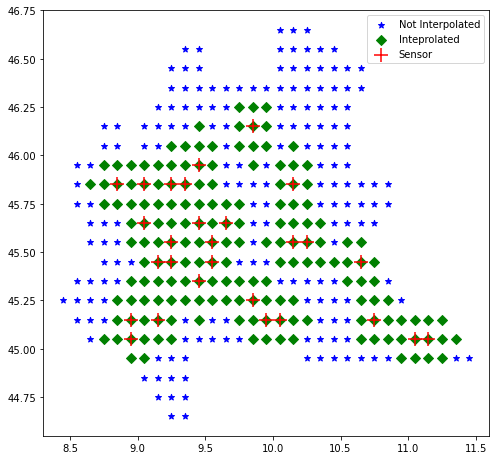
\includegraphics[scale=0.45]{images/buffer.png}}
 { \caption{Graphical representation of how buffer values interpolated from PM2.5 sensors provided by ARPA are added through k-nearest neighbour.}}
\end{figure}

\bigbreak
\subsection{Remove of variables with low variance}
An approach for removing columns is to consider the variance of each column variable. The variance is a statistic representing the expected value of the squared deviation from the mean of a given variable X $\mu$. 
\begin{equation}
  Var(X) = E[(X-\mu)^2]
\end{equation}
The variance can be used as a filter for identifying columns to be removed from a given dataset. 
Using a feature with low-variance only adds complexity and noisy to the feature selection and the predictive.\newline
In order to do that, I performed VarianceThreshold method from the scikit-learn library. In this way, features under a certain variance threshold value should be meaningless and consequently discarded by its dataset. 
\pagebreak
\section{Data Transformation}
Having input variables with different units (e.g. ug/m\textsuperscript{3}, °C, hours or mol/m\textsuperscript{2}) implies data at different scales. This could raise the difficulty of the problem being modelled. \newline
Hence, a common scale through Normalization or Standardization is needed in order to improve the data quality.\newline
Many ML and regression algorithms perform better when numerical input and output variables are scaled to a common standard range. \newline
For instance, it's proved that neural networks trained with scaled data performs better in terms of MSE \cite{shanker1996effect}.
In this step, two type of transformation have been done:
\subsection{Standardization}
The most common data transformation is to centre and scale the each variable values. In order to do that, the average value is removed from all the values. As a result of centring, the predictor will have a zero mean.\cite{kuhn2013applied}
Standardization consists in rescaling data following a gaussian distribution of values with mean equals to 0 and standard deviation equals to 1:
\begin{equation}
  Z = \frac{X-\mu}{\sigma}
\end{equation}
\begin{equation}
\mu = \frac{(\sum_{n=1}^{N} X_i)}{N}
\end{equation}
\begin{equation}
\sigma = \sqrt{\frac{(\sum_{n=1}^{N} X_i-\mu)}{N-1}}
\end{equation}
Where:
\begin{itemize}
\item Z is the numeric value standardized of a given covariate;
\item X is the numeric value to be standardized of a given covariate;
\item $\mu$ is the mean value for the set of values assumed by a given covariate;
\item $\sigma$ is the standard deviation for the set of values assumed by a given covariate;
\end{itemize}
Every terms was computed by using Scipy library (scipy.stats). 
\bigbreak
\subsection{Normalization}
Data Normalization is a different methods process for adjusting data at different scales. Data a scaled in a range between 0 and 1 and was performed only for the feature selection methods output.
Output normalization is an essential step for the comparison of different output, since data ranges vary for each method used.\newline
This was performed in my Notebooks from the scikit-learn library (sklearn.preprocessing) through the MinMaxScaler method.

\section{Feature Selection}
After the previous steps, in which a dataset is cleaned and transformed, FS methods are performed. The output results consist in, for each method a set of score for each variable. The score evaluated corresponds to the importance weighted of each feature with respect to the target variable.
In the following subsection each FS method implemented is described in detail, classified in three main categories\cite{stanczyk2015feature}, as we can find in literature:
\subsection{Filter Methods}
Filter-based feature selection methods adopt statistical measures to evaluate the correlation/dependence between input variables.\newline
These select features from the without machine learning algorithm. In terms of computation, they are very fast and are very suitable in order to remove duplicated, correlated, redundant variables\cite{saeys2007review}. \newline
These methods evaluate each feature individually without considering the interaction between them. Therefore, they don't fit well if data has high multicollinearity\cite{daoud2017multicollinearity}.

\subsubsection{Pearson coefficient}
Pearson coefficient is one of the most widely used indices for measuring linear correlation in statistics. It ranges between -1 and 1, where:
\begin{itemize}
\item 1 indicates a strictly positive correlation;
\item -1 indicates a strictly negative correlation;
\item0 indicates no correlation between the features;
\end{itemize}

Therefore, by taking only its absolute value, 1 implies that a linear equation describes the relationship between X and Y perfectly, for both positive and negative correlation. \newline
The Pearson index between and independent variable X and a target variable Y is defined by the following formula:

\begin{equation}
  \rho_{x,y} = \frac{Cov(X,Y)}{\sigma_x\sigma_y}
\end{equation}

\subsubsection{Kendall Tau}
Kendall Tau index is used to measure monotonic relationship as test statistic to determine whether two variables are statistically dependent. \newline
While in the linear correlation two variables move together at a constant rate, monotonic or rank correlation measure how likely two variables move in the same direction, but not necessarily in a constant manner. \newline
Like Pearson’s correlation, Kendall’s has a value between -1 and 1, where:

\begin{itemize}
\item -1 represent a strictly negative monotonic relationship;
\item 1 represent a strictly positive monotonic relationship;
\item 0 representing no relationship;
\end{itemize}
Given a sample X and Y with n as sample size, tau index is computed through the formula:
\begin{equation}
  \tau_{x,y} = \frac{n_c-n_d}{\frac{1}{2}n(n-1)}
\end{equation}
where:
\begin{itemize}
\item n\textsubscript{c} = \# of concordant value (concordant value: value are ordered in the same way);
\item n\textsubscript{d} = \# of discordant value (discordant value: value are ordered differently);
\end{itemize}
\subsubsection{Spearman Rho}
Spearman’s index is very similar to Kendall’s. As the previous filter methods, it ranges between -1 and 1, and it's considered less robust than Kendall's.
It's computed in this way:
\begin{equation}
\rho_{x,y} = \frac{6\sum_{n=1}^{N} d_i^2}{n(n-1)^2}
\end{equation}
\begin{itemize}
\item d\textsubscript{i}: difference between each corresponding X\textsubscript{i} and Y\textsubscript{i};
\item n: size of the sample;
\end{itemize}

Finally, as I did for Pearson and Kendall coefficient, I take in consideration only its absolute value to weight the correlation for each variable in the Feature Selection.

\subsubsection{Fisher Score}
This method returns the score of the variables based on the fisher’s score in descending order. \newline
Its algorithm is implemented by using SelectKBest method from the scikit-learn library (sklearn.feature\_selection).
\pagebreak
\subsection{Wrapper Methods}
Wrapper methods, as the name suggests, wrap a machine learning model, with different subsets of input features. In this way the subsets are evaluated following the best model performance.
One disadvantage of this approach is the computational costs.\newline
Their execution for many subsets of variables can become unfeasible. 
\bigbreak
\subsubsection{Random Forest Importance}
Feature importance is a built-in function of the Random Forest algorithm. It's also called as Gini importance (or mean decrease impurity) and is commonly used as the splitting criterion in decision trees problem. The scores are evaluated as attribute through RandomForestRegressor of the scikit-learn library (sklearn.ensemble).
\bigbreak\bigbreak\bigbreak
\subsection{Embedded Methods}
Embedded methods instead are characterised by the benefits of both the wrapper and filter methods, by including interactions of features but also having a reasonable computational cost.\par
\bigskip
\subsubsection{Recursive Feature Elimination}
RFE is a wrapper feature selection algorithm that also work with filter-based feature selection internally.\newline
It consists in looking for the best subset of features by starting with all features and removing some of them until the desired number remains.\newline
This is computed using RFE of scikit-learn library (sklearn.feature\_selection).
In order to obtain a score for each variable I consider the ranking value (with ranking\_ attribute) which represent the ranking position for each feature. 
\pagebreak
\subsection{Borda Count: averaging FS results}
One of the most important challenges in this study is the lack of an universal feature selection method which produces an outcomes in common with all FS technique. Choosing a feature selection method from a vast range of choices can be challenging. \newline
So it needs an ensemble technique aims to makes it more robust across various algorithms. In this work we adopt an ensemble approach described in this study\cite{sarkar2014robust}, using the Borda Count algorithm. Initially Borda Count was a voting system method, named for Jean-Charles de Borda\cite{borda1784memoire}.\newline
In this context Borda Count is used as a rank-based combination technique used for evaluate an average score for each feature. In this method, assuming that each scores evaluated by each FS method are sorted in descending order, points are assigned to candidates (variables) based on their ranking; 1 point for last choice (the most meaningless by its score), 2 points for second-to-last, and so on. Finally the points for all ballots are summed up, and the candidates with the largest point total are the winners (the feature with the largest points are the most significant).
\par
At this point variables that won are used as input in ML models and taken in consideration as the most meaningful factor affecting the target variable.
\bigbreak\bigbreak\bigbreak

\section{Notebook implementation for Feature Selection}
A notebook is implemented for processing and analysing data as I explain before.\newline
\begin{comment}

At the beginning the general parameter needed to configure the pre-processing phase are declared.
\begin{verbatim}
RESOLUTION= '0_1' //resolution of the data chosen
KNN = True    //If true a k-nearest neighbour is performed
knn_value = 10 //Number of buffer values added close to each target variable value
NO_MOUNTAINS = True 
\end{verbatim}
\end{comment}
In order to manage its configuration and the results obtained, a simple User Interface using ipywidgets package is built.
In this interface there are 2 sections:
\begin{itemize}
\item Feature Selection scores: they are graphically shown using multiple barplot, one for each dataset previously selected. Barplot are implemented with the use of Plotly library; 
\item Options: in this s box is possible to configure the feature selection input:
\begin{itemize}
\item target variable. Variable usable are the ones coming from ARPA ground sensors;
\item value of the Variance Threshold for discarding meaningless variable before FS (optional);
\end{itemize}
and the output:
\begin{itemize}
\item choice of method for visualize its own scores;
\item results normalization (optional);
\item order of the scores by descending order or by labels;
\item scale of Y-axis (regular or logarithmic);
\end{itemize}
\end{itemize}

\begin{figure}[H]
    \centering
    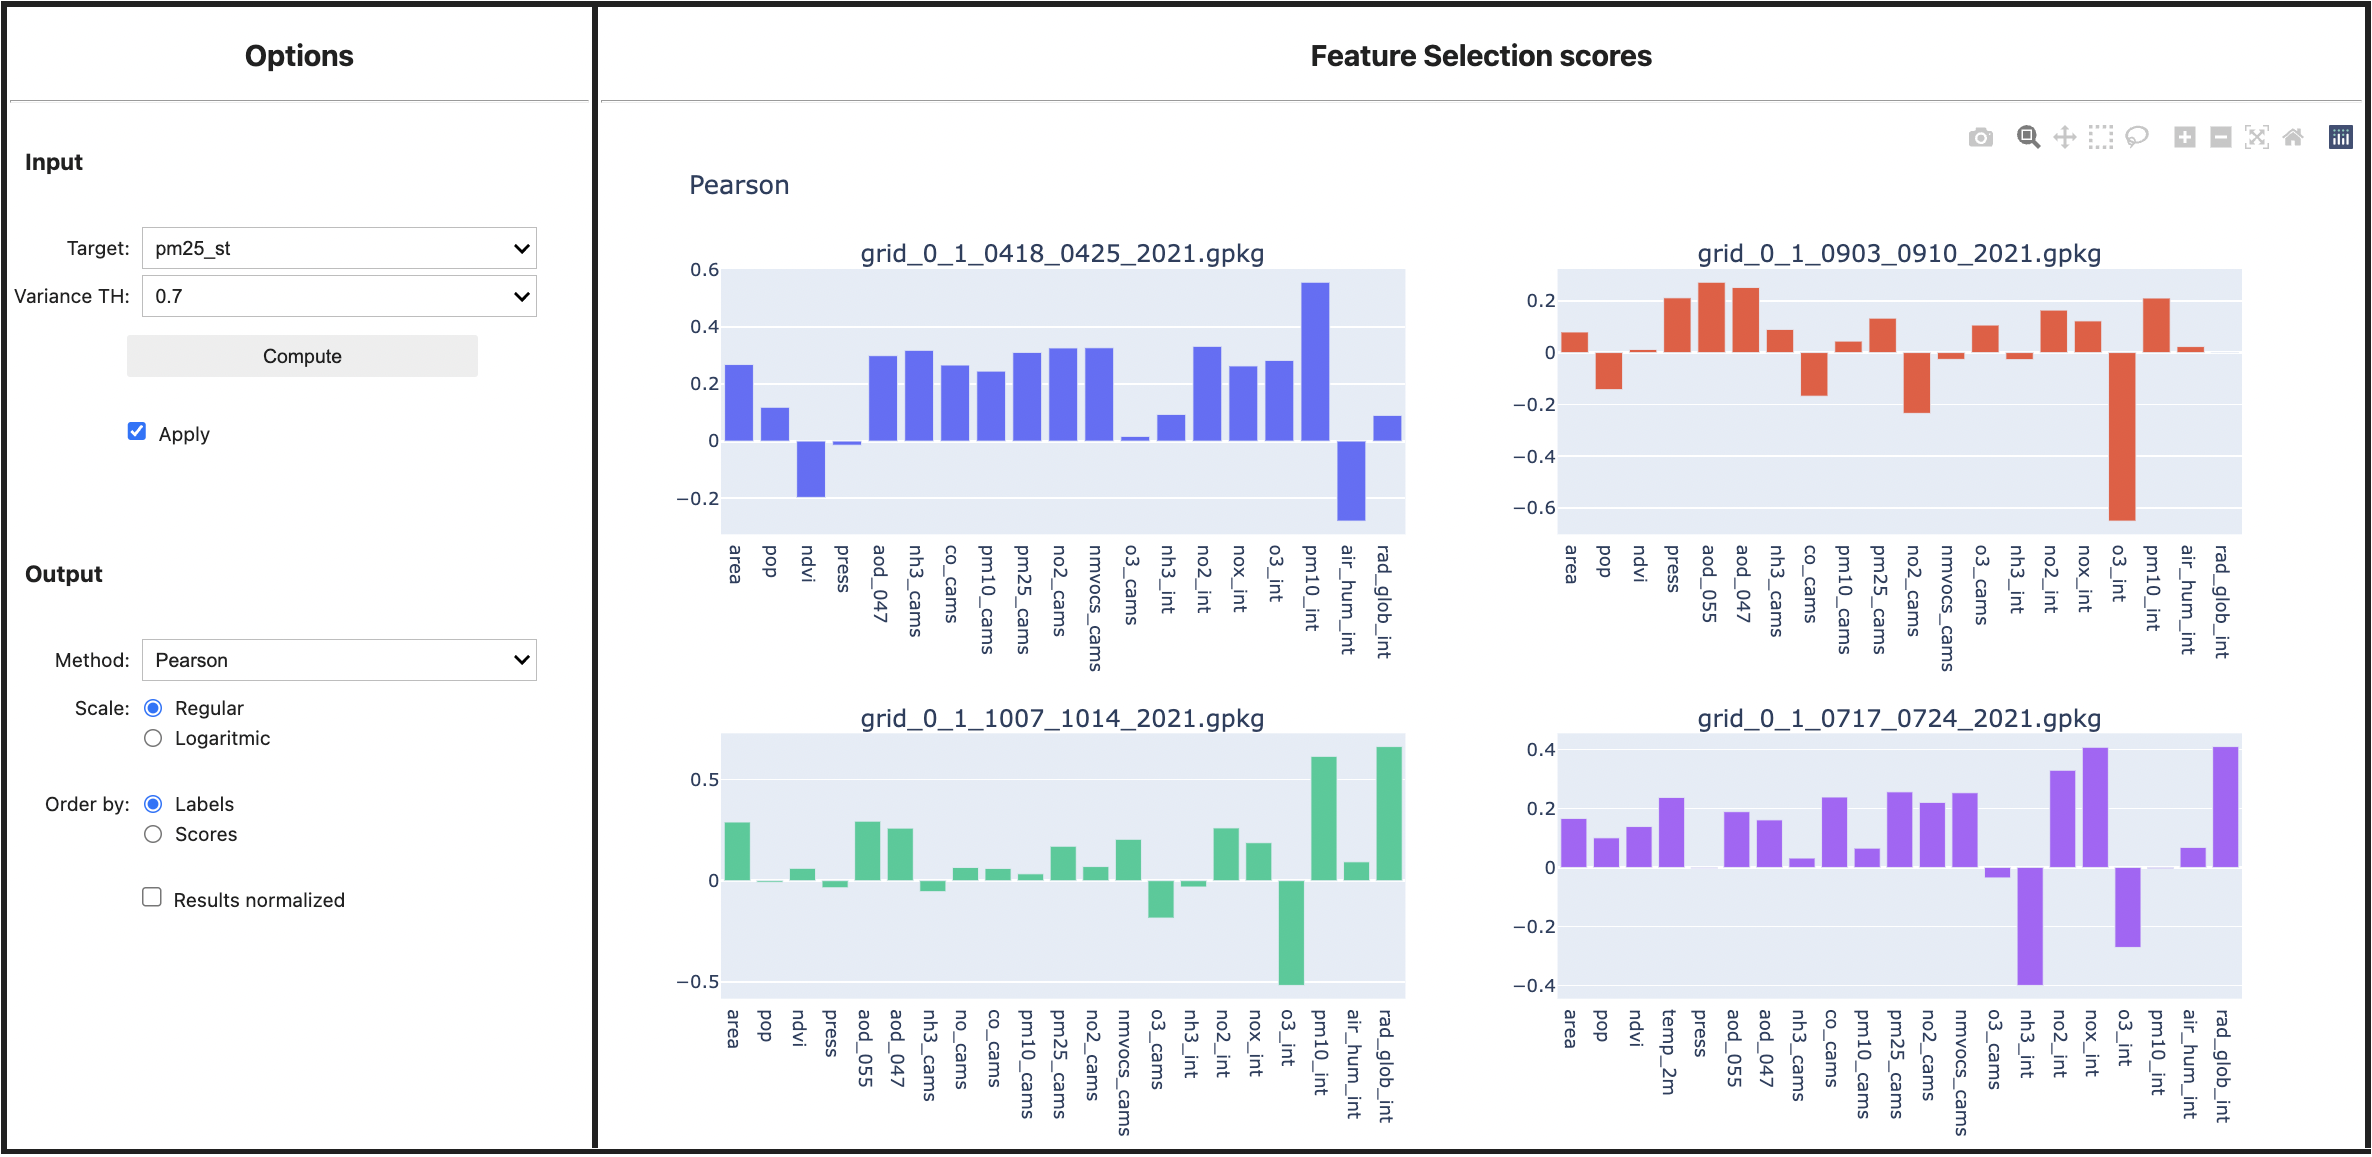
\includegraphics[scale=0.40]{images/notebook.png}
    \caption{Overview of the notebook implemented for FS procedure.}
    \label{fig:notebook}
\end{figure}

